\documentclass{beamer}
\usepackage[T1]{fontenc}
\usepackage[utf8]{inputenc}
\usepackage{lmodern}
\usepackage[ngerman]{babel}

\usepackage{graphics}

\usepackage{amsmath}
\usepackage{booktabs}
\usepackage{listings}

\usepackage{dot2texi}
\usepackage{tikz}
\usetikzlibrary{arrows,shapes}
 \usetikzlibrary{matrix}
\usetikzlibrary{automata}

\usepackage{wrapfig}

\usetheme{Singapore}
\usecolortheme{dove}
\graphicspath{{images/}{../comics/}}

\newcommand{\xn}{\visible<2->{$\times$}}
\newcommand{\xj}{\visible<2->{$\checkmark$}}
\newcommand{\rd}[1]{\textcolor{red}{#1}}
\newcommand{\gn}[1]{\textcolor{green}{#1}}
\newcommand{\bl}[1]{\textcolor{blue}{#1}}

\newcommand{\hiddencell}[2]{\action<#1->{#2}}

\newcommand{\link}[2][blue]{\underline{\textcolor{#1}{#2}}}
\renewcommand{\emph}[1]{\textit{\textcolor{gray}{#1}}}
\newcommand{\warn}[1]{\textcolor{red}{#1}}
\newcommand{\ans}[2]{\visible<#1->{\textcolor{green!70!black}{#2}}}
\newcommand{\wrong}[2]{\visible<#1->{\textcolor{red!70!black}{#2}}}
\newcommand{\xb}[1]{{\bf #1}}   % \xb {fett}
\newcommand{\xu}{\underline}    % \xu {unterstrichen}
\newcommand{\hide}{\onslide+<+(1)->}

\AtBeginSection[]
{
  \begin{frame}[plain]
    \frametitle{}
    {\footnotesize
      \tableofcontents[currentsection]
    }
  \end{frame}
}

\title{Grundbegriffe der Informatik}
\author{Patrick Niklaus}

\begin{document}
\begin{frame}
  \frametitle{Grundbegriffe der Informatik}
  \framesubtitle{12. Tutorium}
  \begin{description}
    \item \textbf{Name:} Patrick Niklaus
    \item \textbf{E-Mail:} patrick.niklaus@student.kit.edu
    \item \textbf{Nr:} 43
  \end{description}
\end{frame}

\section{Übungsblatt}
\begin{frame}
  \frametitle{Anmerkungen zum letzten Übungsblatt}
  \begin{enumerate}
    \item Turingmachinen lieber als Graph angeben
    \item Startzustand nicht vergessen!
    \item Beachtet die Vorbedingung die ein Algorithmus hat um zu funktionieren!
  \end{enumerate}
\end{frame}

\section{Kongruenzrelationen}
\subsection{Was ist das?}
\begin{frame}
	\frametitle{Kongruenzrelationen}
	\begin{definition}
		Äquivalenzrelationen $\equiv$ auf einer Menge M, die mit den Operationen auf M "`verträglich"' sind, nennt man \emph{Kongruenzrelationen}.
	\end{definition}
  \begin{block}{Verträglichkeit}
    $\equiv$ heißt \emph{verträglich} mit $f:M\to M$ wenn gilt:
    $$\forall x_1, x_2 \in M: x_1\equiv x_2 \Rightarrow f(x_1)\equiv f(x_2)$$
    $\equiv$ heißt \emph{verträglich} mit $\diamond:M \times M \to M$ wenn gilt:
		$$\forall x_1,x_2,y_1,y_2: \in M: x_1\equiv x_2 \wedge y_1\equiv y_2 \Rightarrow x_1\diamond y_1 \equiv x_2 \diamond y_2$$
	\end{block}
\end{frame}
\begin{frame}
	\frametitle{Kongruenzrelationen}
	\begin{block}{Zeigt, dass die Äquivalenzrelationen "modulo n" mit + verträglich sind}
		Tipp: $a\equiv b \iff a-b = k\cdot n$
	\end{block}
\end{frame}
\subsection{Ist die Äquivalenzrelation von Nerode eine Kongruenzrelation?}
\begin{frame}
	\frametitle{Ist die Äquivalenzrelation von Nerode eine Kongruenzrelation?}
	Sei \emph{$w'\in A^*$} ein beliebiges Wort und \emph{$f_{w'}:A^*\to A^*$} die Abbildung, die $w'$ an ihr Argument anhängt.\\	
	\begin{proof}
		\textbf{Behauptung:} $\equiv_L$ ist mit allen $f_{w'}$ verträglich.
		$$\forall w_1, w_2\in A^*:w_1\equiv_L w_2 \Rightarrow w_1w'\equiv_L w_2w'$$
		$$\forall w_1, w_2\in A^*:w_1\equiv_L w_2 \Rightarrow f_{w'}(w_1) \equiv_L f_{w'}(w_2)$$
	\end{proof}
\end{frame}
\begin{frame}
	\frametitle{Was sagt uns das jetzt?}
	\begin{block}{Folgerung}
		Wenn man eine Kongruenzrelation $\equiv$ auf $M$ vorliegen hat, die mit einer Operation/Abbildung auf $M$ verträglich ist, wird eine Operation/Abbildung auf $M_{/\equiv}$ induziert.
	\end{block}
	\pause
	\begin{exampleblock}{Beispiel}
		Wir haben gerade gezeigt: $f_x:A^*\to A^*:w\mapsto wx$ ist mit $\equiv_L$ verträglich.\\
		\pause
		Dann ist ${f'}_x:A^*_{/\equiv_L}\to A^*_{/\equiv_L}:[w]\mapsto[wx]$ \emph{wohldefiniert}.
	\end{exampleblock}
	\pause
	\begin{alertblock}{Ganz wichtig!}
		${f'}_x$ ist wirklich \emph{nur} wohldefiniert, wenn die Operation mit $\equiv$ verträglich ist.
	\end{alertblock}
	
\end{frame}

\section{Halbordnungen}
\subsection{Was ist eine Halbordnung?}
\begin{frame}
	\frametitle{Definition}
	\begin{definition}
		Eine Relation $R\subseteq M\times M$ heißt \emph{Halbordnung}, wenn sie folgende Eigenschaften besitzt:
		\begin{description}
			\item[Reflexivität:] $\forall x \in M: xRx$
			\item[Antisymmetrie:] $\forall x,y \in M: xRy \wedge yRx \Rightarrow x = y$
			\item[Transitivität:] $\forall x,y,z \in M: xRy \wedge yRz \Rightarrow xRz$
		\end{description}
	\end{definition}
\end{frame}
\begin{frame}
	\frametitle{Aufgaben}
		Sind die folgenden Relationen Halbordnungen? Wenn nein, welche Bedingungen erfüllen sie nicht?
		\begin{enumerate}
			\item Die Mengeninklusion $\subseteq$ \ans{2}{Ja}
			\item Die Relation $x\equiv y (\text{mod }5)$ \wrong{3}{Nein}
			\item Die Relation $\sqsubseteq_p$ ($w_1\sqsubseteq_pw_2\iff\exists u\in A^*:w_1u=w_2$) \ans{4}{Ja}
			\item Die Relation $a|b \iff \exists n\in \mathbb{N}:a\cdot n=b$ \ans{5}{Ja}
			\item Die Relation $w_1\sqsubseteq w_2 \iff |w_1|\leq |w_2|$ \wrong{6}{Nein}
		\end{enumerate}
\end{frame}
\subsection{Hasse-Diagramm}
\begin{frame}
  \frametitle{Hasse-Diagramm}
	\begin{definition}
		Ein \emph{Hasse-Diagramm} ist der Graph der Relation R ohne $\dots$
    \begin{itemize}
      \item reflexive
      \item transitive
    \end{itemize}
    Kanten.
  \end{definition}
\end{frame}
\begin{frame}
  \frametitle{Aufgabe}
  Zeichnet das Hasse-Diagramm zur Relation $\sqsubseteq_p$, die definiert ist als:$$w_1\sqsubseteq_pw_2\iff\exists u\in A^*:w_1u=w_2$$ auf der Sprache $\{w|w\in \{a,b\}^* \wedge |w|\leq 2\}$.
\end{frame}
\subsection{Extreme Elemente}
\begin{frame}
	\frametitle{Extreme Elemente}
	Es sei $(M,\sqsubseteq)$ eine halbgeordnete Menge und $T$ eine Teilmenge von $M$.\\
  $x \in T$ heißt $\dots$
	\begin{description}
		\item[minimales Element:] $\neg(\exists y\in T: y\sqsubseteq x \wedge y\neq x)$.
		\item[maximales Element:] $\neg(\exists y\in T: y\sqsupseteq x \wedge y\neq x)$.
		\item[kleinstes Element:] $\forall y\in T: y\sqsupseteq x$.
		\item[größtes Element:] $\forall y\in T: y\sqsubseteq x$.
	\end{description}
\end{frame}
\begin{frame}
	\frametitle{Aufgabe}
		Zeichnet ein Hassediagramm, bei dem eine Teilmenge ein minimales Element, aber kein kleinstes Element hat,
		sowie ein maximales Element, aber kein größtes Element hat.
\end{frame}
\begin{frame}
	\frametitle{Extreme Elemente}
	\begin{alertblock}{Beachtet:}
		\begin{itemize}
			\item Wie viele kleinste Elemente kann es geben? \ans{2}{1}
			\item Ist jedes kleinste Element auch ein minimales Element? \ans{3}{Ja}
			\item Ist jedes minimale Element auch ein kleinstes Element? \wrong{4}{Nein}
		\end{itemize}
	\end{alertblock}
\end{frame}

\section{Ordnungen}
\begin{frame}
	\frametitle{Ordnungen}
	\begin{definition}
		Eine \emph{Ordnung} ist eine Halbordnung für die zusätzlich gilt:
		$$\forall x,y\in M: xRy \vee yRx$$
	\end{definition}
\end{frame}
\begin{frame}
	\frametitle{Beispiele}
	\begin{exampleblock}{Lexikographische Ordnung I}
		Die Relation \emph{$\sqsubseteq_1$} sei die Ordnungsrelation, nach der z.B. die Wörter in einem Wörterbuch geordnet sind.\\
		Ergänze:
		\begin{itemize}
			\item aa \visible<2->{$\sqsubseteq_1$} aabba
			\item bba \visible<3->{$\sqsupseteq_1$} aa
			\item aaaaa \visible<4->{$\sqsubseteq_1$} bba
			\item aab \visible<5->{$\sqsupseteq_1$} aaaab
		\end{itemize}
	\end{exampleblock}
\end{frame}
\begin{frame}
	\begin{exampleblock}{Lexikographische Ordnung II}
		Die Relation \emph{$\sqsubseteq_2$} sei die Ordnungsrelation, die zuerst nach Länge und danach alle gleich langen Wörter wie im Wörterbuch ordnet.\\
		Ergänze:
		\begin{itemize}
			\item aa \visible<2->{$\sqsubseteq_1$} aabba
			\item bba \visible<3->{$\sqsupseteq_1$} aa
			\item aaaaa \visible<4->{$\sqsupseteq_1$} bba
			\item aab \visible<5->{$\sqsubseteq_1$} aaaab
		\end{itemize}
	\end{exampleblock}
\end{frame}

\section{Abschluss}
\subsection{Zusammenfassung}
\begin{frame}
  \frametitle{Was ihr jetzt wissen sollte.}
  \begin{enumerate}
    \item Was ist eine Kongruenzrelation?
    \item Was bedeutet eine Relation und eine Abbildung sind verträglich?
    \item Welche Eigenschaften müssen Halbordnungen erfüllen?
    \item Welche Eigenschaften müssen Ordnungen zusätzlich erfüllen?
  \end{enumerate}
\end{frame}

\subsection{xkcd}
\begin{frame}[plain]
  \begin{figure}
    \begin{center}
      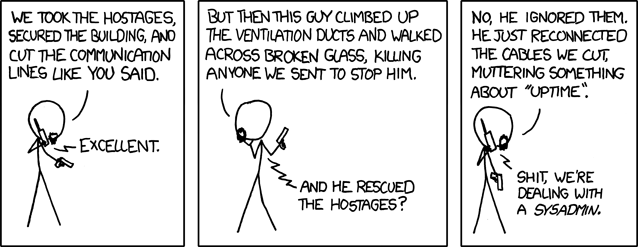
\includegraphics[width=300pt]{devotion_to_duty}
    \end{center}
  \end{figure}
\end{frame}

\end{document}
